% !TEX root = ../main.tex

\chapter{绪论}

\section{研究背景与意义}

% 这是一个提纲
% 1.编排在开发中的地位
% 2.编排的作用是什么
% 3.自动化编排的意义
% 4.LLM赋能自动化编排

近年来,人工智能在经济发展和社会治理中展现了广泛的应用潜力。《中华人民共和国国民经济和社会发展第十四个五年规划和2035年远景目标纲要》明确提出,未来十年内,人工智能将在关键核心技术方面取得重大突破,推动智能化在各个领域的应用。“十四五”期间提出的三大人工智能发展布局——突破核心技术、打造数字经济新优势、营造良好数字生态——为多个行业的智能化升级奠定了坚实的基础。

在这一大背景下,随着大语言模型(Large Language Model, LLM)的快速发展,其在智能系统构建中的应用价值愈发显著。通过将LLM与不同领域的工具集成,可以有效提升用户体验和系统效率。现在许多工具和服务如今都以API(Application Programming Interface,应用程序编程接口)的形式提供,这为智能系统的开发和集成带来了极大的便利。
API作为连接不同系统的通信桥梁,允许开发者在无需了解工具或服务具体实现细节的情况下,直接调用其功能或访问相关数据。

集成了外部工具或在推理规划、记忆方面进行集成的大语言模型应用被称为大语言模型智能体。在复杂场景中,大语言模型驱动的智能体可以集成多种有关工具API,识别自然语言的用户需求并灵活调用工具,为用户提供高效的解决方案。
这种多工具协同能力让智能系统更能适应复杂任务。而在这种协作机制中,编排技术起到了关键作用。

编排的核心在于根据任务目标,对不同的工具、模块或服务进行组织与协调。通过拆解复杂任务为多个子任务,并利用工具间的逻辑关系和数据流动,编排实现了多工具协同工作和复杂任务的自动化执行。这不仅是多工具集成的关键技术,也是提升系统自动化和智能化水平的重要手段。通过编排,系统能够在单一工具的基础上构建更高层次的组合功能,同时确保数据交互和逻辑调用的准确性,尤其在动态需求或复杂任务逻辑下,能够显著提升任务执行的效率和精度。

传统的编排实现中,不同工具之间的接口适配依赖人工定义和开发。开发者需要明确设计工具之间的数据传递逻辑,并手动编写适配代码来实现数据格式的转换和兼容。
这种方式不仅耗时费力,而且难以适应复杂多变的场景。

大语言模型是经过海量数据训练得到的语言模型,具有数十亿到百亿的参数级,具有出色的语言理解能力和生成能力。在工具编排和调用场景下,
大语言模型能够很好地理解用户的任务,并通过工具文档等资源理解工具的作用和能力,最终辅助系统进行编排调度。
引入大语言模型后,能够很好地解决传统编排在灵活性不足、开发门槛高上的问题。大语言模型凭借其强大的语义理解和生成能力,能够在缺乏明确工具调用路径定义的情况下,基于用户目标实时推断任务执行流程。它可以识别工具间的依赖关系,根据依赖关系编排工具调用顺序,并根据任务上下文动态调整工具的输入输出格式。通过自动生成接口适配逻辑,大语言模型大幅降低了人工编写代码的复杂性,降低了编排的技术门槛。同时,LLM还能根据环境的动态变化实时调整任务规划,使系统更高效地应对需求的不确定性和变化。

然而,大语言模型在工具编排领域的应用仍然面临着以下两方面的问题。

% 1.推理和规划能力需要提升,对于大规模的工具候选集的情况难以处理
% 2.对于复杂的工具依赖关系难以处理

\begin{itemize}
    \item 针对大规模工具集时的选择:当面对大规模的工具候选集时,大语言模型的推理和规划能力存在显著不足。
    首先,随着工具数量的增加,模型在从众多工具中筛选出合适工具组合时,选择的难度急剧上升,导致容易选择错误的工具或者是出现”幻觉“现象,如选择不存在的工具。
    此外,大语言模型缺乏对多步骤复杂任务的全局规划能力,其生成的调用路径通常停留在局部优化阶段,而无法兼顾任务的整体逻辑完整性和效率,难以支撑复杂任务的工具协作。
    \item 对复杂工具依赖关系的处理能力不足:多工具协作的任务中,工具之间复杂的依赖关系进一步增加了模型编排的难度。一般来说,大模型工具调用都是通过工具的文档来进行功能理解、参数配置等任务,
    大模型在根据文本识别工具依赖关系时的能力有限,例如,当一个工具的输出需要经过特定处理才能作为另一个工具的输入时,大语言模型难以仅从工具文档中捕捉到这一逻辑,导致工具路径选择不全、或是工具执行顺序出错。
\end{itemize}


% 大语言模型(LLM)尽管展现出强大的语义理解和生成能力,但其固有的“幻觉”(生成不准确或虚假信息)以及“黑盒”性质(缺乏可解释性)在复杂任务中仍然是重要的障碍。这些问题限制了LLM在逻辑推理和内容可靠性上的表现,特别是在多工具协同的场景下,生成结果往往缺乏清晰的依据和可验证性。因此,引入结构化的知识图谱成为解决这些挑战的一种有效路径。
% 
% 知识图谱作为一种领域知识的结构化表达形式,在过去主要用于构建实体及其关系网络,通过命名实体识别、关系抽取和事件抽取等步骤实现精准的信息检索和问答。然而,这些操作通常依赖专家设计规则和手动构建,不仅耗时费力,还难以适应复杂多变的语境。借助LLM强大的语义理解能力,知识图谱的构建效率得到了显著提升。LLM能够从文本中自动提取实体和关系,使知识采集和结构化过程更加智能高效,同时显著扩展了知识图谱的覆盖范围。
% 
% 通过将知识图谱与LLM结合,系统在多工具协同场景中的能力得到了进一步提升。知识图谱的结构化特性为LLM提供了逻辑和语义上的补充,帮助模型动态识别工具间的关联关系并规划调用路径。这种结合弥补了LLM在逻辑推理上的不足,为工具协同提供了一种透明且可验证的逻辑框架。同时,知识图谱还能通过提供约束条件,避免LLM生成幻觉信息,使其内容更加精准和可信。这不仅提升了系统的可靠性,还增强了生成结果的可解释性与用户信任度。
% 
% 尽管大语言模型智能体和知识图谱在工具调用和集成方面展现出巨大的潜力,但仍面临一些关键挑战。第一是大规模工具集成的困难。虽然当前系统可以调用多种API,但随着工具数量的增加,系统需要处理不同的数据格式、调用方式和响应速度,这对模型的调用能力和协调效率提出了更高要求,限制了其在复杂场景中的适应性与灵活性。第二是工具间复杂依赖关系的处理难题。在需要多个工具协同工作的任务中,模型常常难以有效管理工具间的依赖关系。例如,一个工具的输出需要作为另一个工具的输入时,调用顺序和逻辑必须精确无误。然而,目前的大语言模型在协调这些复杂依赖关系方面能力有限,可能导致任务中断或结果误差。

\section{国内外研究现状}

本节将概述针对大语言模型工具图谱与智能体工具调用的研究进展。

% 工具图谱能对工具之间的依赖关系进行表示和存储,
% 通过在工具知识图谱上搜索工具路径能够得到调用路径。
% 但是图上固有的工具路径有时不能满足变化的用户需求。
% 同时,从用户输入的自然语言需求到根据工具进行回复的过程中,有许多步骤都需要大语言模型参与。
% 使用大语言模型进行选择和编排能够提升系统的动态性和灵活性,但仅依赖大语言模型的语义分析能力难以处理工具之间的复杂依赖关系。
% 因此需要结合。。。

首先,本节会介绍大语言模型智能体工具调用方面的研究,
包括不同的多智能体协作流程和提示词工程的方法,详细描述各种提升模型在工具编排、工具调用方面的能力,以及目前存在的一些待解决的问题。
其次,本节会介绍有关图谱与大语言模型结合的应用场景,特别是工具图谱在大语言模型工具调用上的应用,比如通过对工具之间的时序关系、资源依赖关系建模,从而得到工具调用路径的现有方法和局限性。

\subsection{大语言模型智能体工具调用}

为大型语言模型(LLMs)引入外部工具显著增强了智能体在应对复杂现实任务时的能力\cite{huang2024planning, Qin2023, qu2024tool}。
通过支持功能调用,LLMs 能够获取最新信息、提升专业技能、
执行精确计算并调用第三方服务,同时功能调用也能提高回答生成过程中的透明性和鲁棒性,让回答更具有可解释性和可靠性。
因此大语言模型智能体在多个领域实现了广泛的应用,例如多媒体内容搜索\cite{Song2023}、财务分析\cite{theuma2024equipping}以及旅行规划\cite{hao2024large}。

然而,要充分发挥工具调用的潜力并高效完成复杂任务,必须应对功能调用本身所带来的技术挑战。这些挑战并不仅限于简单的接口调用,而是伴随着实际应用场景的多样化需求和复杂性。例如,从如何管理多种 API 的协作,到如何优化工具调用的顺序和数据依赖关系,这些都对大语言模型的能力提出了更高的要求\cite{huang2024planning, Qin2023}。为深入理解这些问题,我们需要分析功能调用在实际应用中的复杂性及其解决思路。

功能调用的复杂性主要来自实际应用中 API 的多样性、复杂性及其相互依赖的特性\cite{Qin2023}。例如,现实场景中的 API 参数往往不仅限于简单的字符串或数字,还可能包括列表、字典、嵌套结构,甚至这些类型的组合。参数的数量可以从零到几十不等,其应用领域覆盖了多个行业和业务场景\cite{ye2024tooleyes}。此外,为完成一项任务,通常需要多个工具协同工作,单一 API 难以满足复杂任务的需求\cite{huang2024planning}。更复杂的是,一个 API 的输入可能依赖于另一个 API 的输出\cite{Qin2023},进一步增加了功能调用的挑战性和复杂性。

在大语言模型工具调用上,可以通过训练和非训练的方式来提升大语言模型的工具调用能力。
\cite{Qin2023, schick2024toolformer, hao2024toolkengpt, parisi2022talm}等研究者通过微调开源的大语言模型来增强模型的工具能力。
基于训练的方式需要耗费大量的计算资源,并且涉及到数据集的构造和清洗,
最终得到的模型仅适用于特定的领域,使用场景有限。
这些方法还仅适用与开源大语言模型,因为需要修改模型的参数,难以扩展到闭源的黑盒LLMs。
最后,该方法在以“即插即用”方式集成外部工具方面缺乏灵活性。


% 可能需要一个更加流畅的逻辑链条
% 大语言模型工具调用有哪些问题

% 在大语言模型智能体工具调用中,主要会面临一下

大语言模型的工具调用流程通常可以划分为以下四个核心阶段\cite{Ruan2023, Shen2023, Song2023}:任务规划、工具选择、工具调用和响应生成。尽管其他框架可能存在差异,但通常也是在此基础上进行修改、合并或删减。接下来,我们将按照这些模块化分层依次展开介绍。

\subsubsection{工具任务规划}

在现实的信息查询场景中,用户的查询需求往往包含复杂的意图,如何识别用户意图并明确定义好任务是工具调用的首要问题。
因此在工具任务规划阶段,我们首先需要将用户的需求语句转化为更加明确的任务,并对复杂任务进行拆解。

现有研究\cite{Miao2023}表示,大语言模型能够通过少样本甚至零样本实现有效的任务规划。
HuggingGPT\cite{Shen2023}首先把任务分解为各种子任务,然后选择合适的模型来解决这些子任务。
RestGPT\cite{Song2023}引入了一种从粗粒度到细粒度的规划方法,能够指导大语言模型逐步对任务进行分解。

\subsubsection{工具选择}

在任务规划阶段完成后,需要根据每个子任务进行工具选择。工具选择过程一般有两种途径:
一种是通过训练得到的检索器来选择工具,另一种是直接让大语言模型从工具列表中选择合适的工具。

基于检索器的工具选择:当工具数量过多时,通常会使用检索器先搜索得到与任务相关的工具。
检索方式包括基于关键词的检索和基于语义的检索两种。
基于关键词的检索:通过精确匹配实现用户需求和文档之间的对齐和查询,如TF-IDF\cite{Jones1972}和BM25\cite{Robertson2009};
基于语义的检索:利用神经网络来学习文本之间的语义关系,然后使用余弦相似度等算法计算语义相似度,
如ToolLLM\cite{Qin2023},在其中作者们对BERT模型在工具数据集上进行微调,
提升了其在工具检索场景上的能力,进一步增强了基于语义检索的准确性。

基于大语言模型的工具选择:在工具数量有限,或者是已经检索得到少量有关工具时,可以让大语言模型利用自身的推理和分析能力选择最合适的工具。
具体来说,我们可以将备选工具信息与用户需求一起放入大语言模型的输入上下文,提供给模型。随后,模型根据用户需求选择合适的工具。

通用的提示词技巧可以帮助在多个工具中选择正确的工具。Chain of Thought(CoT)\cite{Wang2023a}在提示词中加入了例子,
让大模型在解决复杂问题时采取相应的推理步骤,
让大模型以分步的方式来规划和行动。
Re-Prompting\cite{Raman2022}在生成计划之前会检查每个步骤是否能够执行。
如果不能够执行,则让大模型重新生成计划。Self-consistent CoT(CoT-SC)\cite{wang2022self}因此让大模型执行多条推理路径,
选择出现频率最高的答案输出。
Tree of Thoughts(ToT)\cite{Yao2023a}用树状的形式组织推理过程,
树上的每个节点表示一个“想法”即推理中间步骤。
中间步骤的选择基于大模型的评估,最终计划用深度优先遍历(DFS)或者广度优先遍历(BFS)得出。
在GoT\cite{Besta2023}中,作者把用树状结构组织推理扩展为了用图结构组织。
引入环境反馈同样可以提升能力,ReAct\cite{Yao2023b}中指导大模型按照指定格式来思考和行动。
生成的想法来帮助大模型进行推理和规划,基于这个想法大模型会采取不同的行动,
最后观察该行为的结果并作为反馈提供给大模型。Voyager\cite{Wang2023b}里智能体接收的反馈包括三种:
程序执行的中间结果、执行错误描述和自我验证结果。Inner Monologue\cite{Huang2022}主动获取人类的反馈,
将其与环境反馈进行结合,用于增强大模型的规划和推理能力。
SelfCheck\cite{Miao2023}则让智能体对自己的推理步骤进行检查和评估,根据结果来修改计划以提升性能。

关于专门针对工具选择场景的提示词工程和流程搭建工作,ToolNet\cite{Liu2024}将大量工具组织成为有向图的形式,允许大语言模型从初始节点出发,迭代地在图上选择下一个工具,直到走到标记为结束节点的节点。
ToolLLM\cite{Qin2023}中提出了基于深度优先遍历算法的决策树算法,通过支持回溯操作解决了在工具选择上的错误传播问题,有效提高了整体的准确性和通过率。
AnyTool\cite{Du2024}提出了一种自我反思的层次化选择的方法,通过在结构化的工具调用树上迭代选择合适的工具。

在真实场景中,工具的数量通常非常庞大。如果将所有工具的描述都作为 LLM 的输入,会面临上下文窗口长度限制和模型生成时间延迟的限制。
因此,近期的研究越来越多地关注先通过检索器筛选工具\cite{Qin2023, anantha2023protip, Liu2024} ,再让大语言模型进行选择。

\subsubsection{工具调用}

处理有依赖的工具/任务之间的输入输出也较为复杂。在ReWOO中\cite{xu2023rewoo},作者提出通过占位符替代的方式来表达工具之间的参数传递,即用占位符来表示工具之间的参数依赖关系,待前序工具调用成功后将后续工具的输入中的占位符替换为前序工具的输出。然而,现实生活中,工具API的输入和输出可能包括字符串、列表、嵌套结构等多种类型,其数量和结构因工具而异,简单的占位符替换无法满足现实场景中的工具调用需求。

在工具调用部分,大语言模型主要负责根据工具描述文件来提取工具调用所需的参数,并对工具服务器请求服务。
这一过程要求 LLMs 不仅能够正确提取参数的内容和格式,还必须严格遵循规定的参数输出来输出。

无需微调的方法主要通过提示词工程、多智能体协作来提升工具调用能力。基于提示词工程的方法利用少样本(few-shot)技术提供参数提取的示例,从而增强 LLM 提取参数的能力\cite{Song2023, Liu2023a, Liu2024, hsieh2023tool}。
Reverse Chain\cite{zhang2023reverse}采用逆向思维,首先为任务选择最终工具,然后让 LLM 填写所需的参数;如果缺少参数,则基于描述选择额外的工具来补全参数,最终完成任务。
EasyTool\cite{yuan2024easytool}通过提示 ChatGPT 重写工具描述,使其更简洁并直接包含工具功能的使用指南,增强 LLM 对工具功能和参数需求的理解。
ConAgent\cite{shi2024learning}引入了一种多智能体协作框架,其中一个专门的执行智能体负责任务执行和工具调用。

\subsubsection{响应生成}

由于工具输出形式多样且复杂,这些结果可能以文本、数字、代码等不同格式呈现,因此无法直接提供给用户查看。需要通过大语言模型(LLM)对这些输出进行组织和分析,围绕用户的查询提取相关信息,并结合模型自身的知识生成完整且清晰的回答。根据将工具输出融入大语言模型提示词的方式,现有方法主要分为直接插入方法和信息整合方法两类。

直接插入方法是早期研究中常见的一种实现方式 \cite{schick2024toolformer, wang2024tools, hao2024toolkengpt}。
模型会首先输出带有占位符的回答,在得到工具调用结果后将占位符替换为工具结果。
然而,由于工具输出结果的形式和内容往往难以预测,这种方法可能会影响用户体验。

为了克服这一问题,许多研究选择将工具输出作为上下文的一部分输入到 LLM,以便生成更高质量的响应 \cite{shen2024hugginggpt,}。
不过,由于 LLM 的上下文长度有限,对于某些工具输出内容,直接输入会面临挑战。
为此,不同方法提出了多种解决方案。例如,RestGPT \cite{Song2023} 通过预定义模式(schema)来简化冗长的工具输出,这些模式包括示例、格式和可能错误的说明文档。
ToolLLaMA \cite{Qin2023} 采用截断策略,将输出裁剪到适当的长度范围内,但可能因此丢失解决用户问题的关键信息。
ReCOMP \cite{xu2023recomp} 提出了一种压缩机制,可以将冗长的工具输出浓缩为简洁的版本,仅保留核心内容。

% 现有的问题:
% 1.针对复杂的自然语言需求处理能力不足(举例ToolLLM的正确率只有40\%不到)
% 这是因为:
% a.幻觉(选择不存在的工具)
% b.任务之间的依赖关系难以处理(找不出这些依赖、对依赖的处理错误、api之间的先后调用顺序和参数)
% c.尽管有一些方法可以解决(比如react prompting技巧,前一个的输出可以放到后一个的输入),但是迭代一次又一次api选择这样又造成了整体花费时间过长,api调用重复/出错/执行过程难以主动结束这些问题。而且这样无法并行调用。
% 2.工具扩展性不足
% a.工具箱扩展性强。因为所有解决方案都依赖于工具图,当工具变化时,只需重建图而无需重新训练LLMs或更新上下文提示。
% b.

% 综上,还有很多工具的问题需要解决。所以需要提出一个更完善的多智能体工具流程来实现这一切。

然而,对于现实世界的复杂需求,现有方法仍然存在显著问题。
首先,复杂任务本身包含多个有相互依赖的子任务,任务编排的复杂性也来自于子任务之间的依赖关系。功能调用的复杂性来源于实际应用中工具的多样性和参数的高度复杂性。
其次,工具之间往往存在复杂的依赖关系,例如一个工具的输入可能依赖于另一个工具的输出。现有模型在表达和处理这种依赖关系时能力不足,常常导致依赖关系无法识别、识别失败等问题,严重影响任务执行的完整性。
此外,现有方法多采用逐步迭代的工具调用方式(如 ReAct 技术\cite{Yao2023b})。虽然通过将先调用工具的响应嵌入后续工具选择和参数提取的提示词上下文中,部分缓解了工具依赖问题,但这种方法也带来了新的挑战:随着调用次数增加,上下文长度不断增长,导致Token消耗量大幅增加。同时,由于工具之间按照线性顺序逐一执行,无法并行化处理,不仅增加了总执行时间,还显著降低了系统效率。
最后,现有工具调用流程的鲁棒性仍然不足。在面对复杂的自然语言需求时,模型可能生成不存在的工具调用(即幻觉现象),或因调用失败无法动态调整任务计划,从而造成任务中断或结果不完整。这些问题严重限制了现有方法在复杂任务场景中的实际效果和扩展性。

\subsection{大语言模型与工具图谱结合的应用}

% 尽管大语言模型主要用于纯文本的场景,但是在许多现实场景中,文本数据与丰富的结构信息以图谱的方式存储。
% 此外,大语言模型的基于文本的推理能力已经得到较多的展现,但是大语言模型在图谱上的推理能力仍有很大的探索空间。

% 通过将现实世界的知识表示为结构化的知识图谱,并在图谱上进行推理和演算,能够解决许多重要问题。

% 关于如何将图谱上的知识提供给大语言模型的问题,有三种常见的方法:

% 自然语言描述。用自然语言描述图结构是最简单的方式,可以直接描述图上的边和邻接列表;对图进行文本上的改写。由于自然语言描述图通常会较为复杂,而且不具备结构化的特点,因此对图的描述进行了改写,得到了更加高效的图的描述,有利于模型对图谱信息的利用;对图进行编码。最后一种方法是通过训练图编码器,将图结构编码成为特征序列并作为特征的一部分输入到大语言模型中。这种方法涉及到对大语言模型的微调,以让其适应新的输入格式。

尽管大型语言模型(LLMs)在广泛任务中取得了显著进展,但在正确使用大量外部工具方面仍存在显著局限性。现有的上下文学习方法仅将工具格式化为一系列纯文本描述,并将其输入到LLMs中,由此生成一系列工具调用步骤以逐步解决问题。这种范式忽略了工具之间的内在依赖关系,并将所有推理负担转移到LLMs上,使其仅限于少量专门设计的工具。因此,当面对真实世界的场景时,LLMs在操作大规模工具库时仍充满挑战,极大地限制了其能力。

通过构建工具知识图谱,将工具之间的依赖信息存储到工具图谱中,再通过在图谱上遍历或搜索图上信息提供给大语言模型智能体,能够显著提升整体的工具调用准确性和效率。

常见的做法是利用深度优先搜索算法(DFS)或者广度优先搜索算法(BFS)来实现在图上的推理和搜索。
许多研究探索了基于搜索的推理,特别是在知识图谱领域。
Reasoning on Graph\cite{Luo2023}的方法将知识图谱作为可靠的知识来源,通过提示大语言模型生成多个关系路径作为计划,
随后根据这些路径不断在知识图谱上搜索,有效地提高了回答的可信度和效率。

另一种方法是在图谱上动态地进行迭代检索和推理子图来模拟动态搜索过程\cite{Liu2024, Sun2023, Ma2024}。
在每个步骤中,大语言模型都检索当前节点的邻居节点,然后决定下一步操作是继续搜索还是结束搜索并给出答案。

% 问题1:如何构建工具图(本体模型、blabla模型)

Think-on-Graph系列\cite{Sun2023,Ma2024}在知识图谱上通过大语言模型Agent进行迭代式的束搜索,探索发现最好的推理路径,
并返回最有可能的推理结果。

ToolNet\cite{Liu2024}中,作者根据工具调用的数据集建立了图谱,并根据图谱上的边进行搜索,迭代式选择所需的工具进行调用,
有效提升了工具搜索的准确性。

ControlLLM\cite{Liu2023a}引入了 “在图上思考”(Think-on-graph, ToG)的范式,通过深度优先搜索算法(DFS)在构建好的工具图上进行搜索,得到解决方案。

GNN4TaskPlan中\cite{wucan2024}通过构建工具图和使用图神经网络,实现了非训练和基于训练的两种方式,
使用图神经网络与当前流行的提示词工程的方法形成了互补,能够有效提升大语言模型在任务规划上的准确性。

%2 问题2:用LLM构建工具图(graphrag blabla)

% GraphRAG\cite{}

尽管现有研究已经初步尝试将工具图谱与大语言模型结合,但在理论和实践上仍然存在显著的局限性,这些问题在实际应用中表现得尤为突出。

\textbf{首先,工具图谱的规模和场景局限性严重限制了其通用性和扩展性。}例如,TaskBench\cite{shen2023taskbench} 所构建的工具图仅包含少量工具节点,工具图谱规模较小,无法表达真实世界的复杂工具调用场景。ControlLLM\cite{Liu2023a} 仅针对多媒体领域的 API 工具接口进行了“资源依赖”的工具图谱建模,缺乏对通用 API 工具场景的支持。在多媒体领域下,工具的输入输出都是单个多媒体文件格式,不像通用API工具一样具有复杂的输入输出格式,这样的研究无法验证在通用场景下工具图谱的效果。
\textbf{其次,现存工具知识图谱中的工具关系建模过于简单,无法真实反映工具间的复杂依赖关系。}大多数工具图谱仅在工具之间构建单一类型的关系,例如在ToolNet中作者仅考虑了工具之间的时序关系\cite{Liu2024},但是这种时序关系是通过分析API调用路径得到的,不具备可解释性,无法明确表示工具之间的依赖。在ControlLLM\cite{Liu2023a}中,作者们对工具之间进行了一种关系的建模,即多媒体资源类别的建模。TaskBench\cite{shen2023taskbench}构建了三个图谱,但是每个图谱中仍然只存在单一的工具依赖关系。当前的工具图谱研究未能将这些工具之间多样化的依赖关系表示在同一个图谱中,局限了工具图谱的适用范围和可解释性。
\textbf{最后,工具图谱的构建策略过于依赖人工与路径数据,未能充分利用现有工具描述文档中的丰富语义信息。}当前方法多依赖手动提取工具之间的依赖关系或基于已有调用路径构建图谱,忽略了工具描述文档中参数、功能和使用示例等隐含的知识。这种做法不仅使得图谱构建过程繁琐且难以扩展,还严重限制了图谱的表达力和适用性。在实际应用中,这类图谱往往难以灵活适配动态变化的工具集或新出现的任务需求,进而影响复杂任务中的工具调用与优化。

综上,这些问题直接限制了现有工具图谱方法在复杂任务场景中的通用性和实用性。面对真实世界中日益复杂的工具编排需求,
现有研究在图谱规模、关系建模和自动化构建能力上都存在较大的改进空间。要促进工具知识图谱与大语言模型工具调用的有机结合,亟需探索如何突破这些局限,从而实现对更大规模、更通用场景的方法。

\section{研究问题}

基于以上的研究背景和现有方法的局限性,本文的核心研究问题归纳如下:
\begin{itemize}
    \item \textbf{如何构建一个工具图谱来表示工具依赖关系?}  
    本问题旨在研究如何利用工具调用路径数据及其工具描述文档,挖掘工具之间的时序关系、参数依赖以及调用逻辑,构建一个支持复杂任务的工具知识图谱。包括如何进行数据筛选和清洗,以保留高质量的工具和工具调用数据;如何实现一个高效的工具关系的自动化建模方法;以及如何通过该图谱提升工具选择和依赖参数配置的准确率与效率。
    
    \item \textbf{如何结合知识图谱与大语言模型智能体设计高效的工具编排与调用框架?}  
    本问题关注如何利用工具图谱与大语言模型,设计一个高效的任务分解、工具选择和工具调用的多智能体框架。
    包括如何准确识别和分解工具之间的复杂依赖关系,并在执行流程中根据这些依赖关系进行工具调用顺序的编排;
    如何获取到合适的一组候选工具集合供工具选择器进行工具选择和参数获取;
    如何通过工具并行化调用和工具响应压缩等方法提升任务执行效率,节省大语言模型的计算开销。
    
    \item \textbf{如何在复杂任务场景中验证上述方法的有效性与优越性?}  
    本问题探讨如何构建实验基准和评价指标,验证所设计智能框架在复杂任务场景中的实际表现。包括如何评估框架在工具调用正确性、任务完成效率、工具选择准确性等方面的性能,以及如何提升其在大规模工具集合和在各种领域的通用性。
\end{itemize}

\section{研究内容}

本文研究与实现的内容主要包括以下几点:

\begin{enumerate}
    \item 本文提出了一种基于规则与大语言模型的工具知识图谱构建方法,对工具领域的关系和实体进行建模和表示。首先,我们通过设计了针对工具文档和针对工具调用路径的两种数据筛选策略,从原始工具数据集中筛选出了高质量的工具集合与有效工具调用路径。其次,我们定义了工具图谱概念模型和层次关系,建模工具之间的时序与资源依赖逻辑。最终,构建并导入Neo4j数据库的高质量工具图谱,实现了可视化与高效查询,为复杂任务的工具调用与规划提供支持。
    \item 为了有效利用构建的工具图谱的知识,本文提出了基于工具图谱和多智能体的工具调用流程和基于DFS的工具调用路径搜索算法。该方法通过在图谱上进行深度优先搜索,能够充分利用工具知识图谱来进行工具选择和执行顺序编排。同时,我们提出了智能体的记忆框架,通过维护历史工具调用知识,进一步辅助大语言模型的规划和推理。我们在真实世界的API测试集上进行充分实验,验证了该方法的有效性,并且证明该方法优于基线方法。
    \item 本文设计并实现了一个基于知识图谱和大语言模型的智能API编排与调用系统,旨在提供用户友好的交互体验。本工作允许用户通过自然语言提问,系统能够解析用户需求、进行工具选择和编排、并根据得到的工具调用路径依次执行API工具。最终,根据API的响应结果生成自然语言格式的回复。该系统有用户登录、API调用路径生成、问答服务以及自定义工具添加等功能,而管理员可以管理模型超参数配置和数据库。系统的整体架构分为存储层、访问层、功能层、接口层和展示层五层,各层负责不同的功能,以确保系统的高效性和易用性。
\end{enumerate}

\section{论文组织结构}

如图\ref{fig:ch1-structure}所示,本论文的内容组织结构分为以下几章:

\begin{figure}[!htp]
    \vspace{1em}
    \centering
    \setlength{\abovecaptionskip}{10pt} % 控制图片和caption之间的距离
    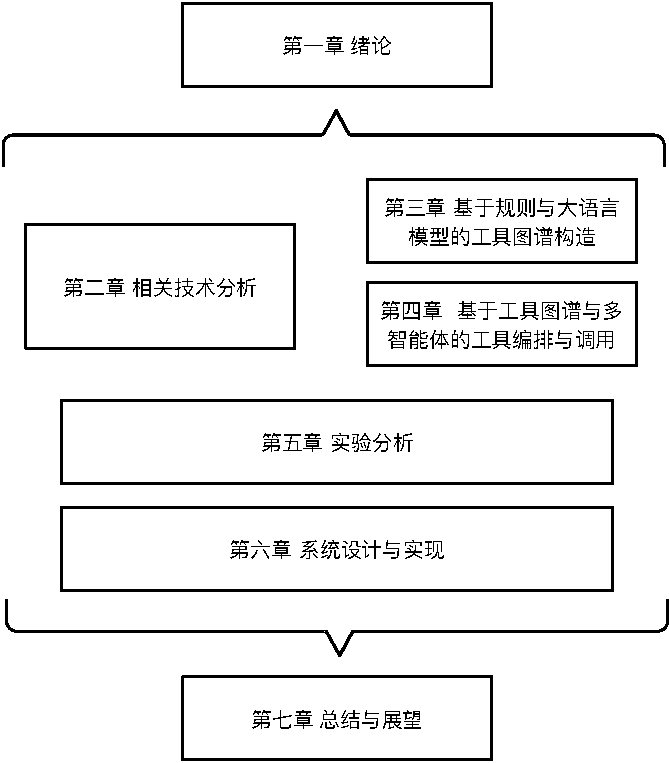
\includegraphics[height=9cm]{../assets/ch1-论文结构.pdf}
    \bicaption{论文组织结构}{Structure of the Paper}
    \label{fig:ch1-structure}
  \end{figure}

  \indent 第一章为绪论,本章从研究背景出发,简要阐述了研究的问题与难点,分析了国内外的研究现状,介绍了本文的主要工作内容,并对全文的组织结构进行了概述。

  \indent 第二章为相关理论与技术,本章主要介绍了研究相关的核心概念与技术背景。首先,介绍了知识图谱的定义、分类及基于API的知识图谱研究;其次,阐述了大语言模型的定义、发展历程及其关键技术,包括大模型智能体、提示词工程和检索增强技术等;最后,探讨了大语言模型与图谱结合的应用方案及其典型案例。
  
  \indent 第三章为规则与大语言模型的工具知识图谱构建方法及实现,本章提出了一种利用规则和大语言模型的知识抽取方法。内容包括对工具数据集的筛选与清洗、图谱概念模型的设计和基于规则和基于大语言模型的工具知识抽取。最终构建了一个完备的工具知识图谱,为后续的工具编排与执行流程提供支持。
  
  \indent 第四章为基于工具图谱与多智能体的工具编排与调用方法的设计与实现,本章聚焦于基于大语言模型智能体的工具任务解决方案,涵盖任务分解、工具选择、工具调用及工具总结等关键流程。同时,针对工具选择阶段,我们提出了一种工具检索器的训练方式,通过两种不同难度的负样本构造方式,训练了一个工具检索器,用于提升工具检索的效率和准确性。
  
  \indent 第五章为实验分析,对本文中提出的方法进行了丰富的实验。本章通过对API检索器模型进行实验,验证了微调模型在工具检索中召回率和NDCG指标的提升。同时,对整体的基于工具图谱和多智能体的API编排与调用流程进行了评估,结果与多个基线方法进行对比,证明了本文方法的可行性与优越性。
  
  \indent 第六章为系统设计和实现,本章在前几章的基础上完成了系统的架构设计和功能模块实现,最终构建了可视化Web界面。具体内容包括系统框架设计、关键功能模块开发及系统展示。
  
  \indent 第七章为总结与展望,本章回顾了全文的研究工作,概括了主要成果,并针对本研究的局限性提出改进方向,展望了未来在知识图谱与大语言模型结合领域的研究前景。